% Options for packages loaded elsewhere
\PassOptionsToPackage{unicode}{hyperref}
\PassOptionsToPackage{hyphens}{url}
%
\documentclass[
  12pt,
]{article}
\usepackage{lmodern}
\usepackage{amssymb,amsmath}
\usepackage{ifxetex,ifluatex}
\ifnum 0\ifxetex 1\fi\ifluatex 1\fi=0 % if pdftex
  \usepackage[T1]{fontenc}
  \usepackage[utf8]{inputenc}
  \usepackage{textcomp} % provide euro and other symbols
\else % if luatex or xetex
  \usepackage{unicode-math}
  \defaultfontfeatures{Scale=MatchLowercase}
  \defaultfontfeatures[\rmfamily]{Ligatures=TeX,Scale=1}
\fi
% Use upquote if available, for straight quotes in verbatim environments
\IfFileExists{upquote.sty}{\usepackage{upquote}}{}
\IfFileExists{microtype.sty}{% use microtype if available
  \usepackage[]{microtype}
  \UseMicrotypeSet[protrusion]{basicmath} % disable protrusion for tt fonts
}{}
\makeatletter
\@ifundefined{KOMAClassName}{% if non-KOMA class
  \IfFileExists{parskip.sty}{%
    \usepackage{parskip}
  }{% else
    \setlength{\parindent}{0pt}
    \setlength{\parskip}{6pt plus 2pt minus 1pt}}
}{% if KOMA class
  \KOMAoptions{parskip=half}}
\makeatother
\usepackage{xcolor}
\IfFileExists{xurl.sty}{\usepackage{xurl}}{} % add URL line breaks if available
\IfFileExists{bookmark.sty}{\usepackage{bookmark}}{\usepackage{hyperref}}
\hypersetup{
  pdftitle={Supplementary Information},
  hidelinks,
  pdfcreator={LaTeX via pandoc}}
\urlstyle{same} % disable monospaced font for URLs
\usepackage[margin=1in]{geometry}
\usepackage{longtable,booktabs}
% Correct order of tables after \paragraph or \subparagraph
\usepackage{etoolbox}
\makeatletter
\patchcmd\longtable{\par}{\if@noskipsec\mbox{}\fi\par}{}{}
\makeatother
% Allow footnotes in longtable head/foot
\IfFileExists{footnotehyper.sty}{\usepackage{footnotehyper}}{\usepackage{footnote}}
\makesavenoteenv{longtable}
\usepackage{graphicx}
\makeatletter
\def\maxwidth{\ifdim\Gin@nat@width>\linewidth\linewidth\else\Gin@nat@width\fi}
\def\maxheight{\ifdim\Gin@nat@height>\textheight\textheight\else\Gin@nat@height\fi}
\makeatother
% Scale images if necessary, so that they will not overflow the page
% margins by default, and it is still possible to overwrite the defaults
% using explicit options in \includegraphics[width, height, ...]{}
\setkeys{Gin}{width=\maxwidth,height=\maxheight,keepaspectratio}
% Set default figure placement to htbp
\makeatletter
\def\fps@figure{htbp}
\makeatother
\setlength{\emergencystretch}{3em} % prevent overfull lines
\providecommand{\tightlist}{%
  \setlength{\itemsep}{0pt}\setlength{\parskip}{0pt}}
\setcounter{secnumdepth}{5}
\usepackage{rotating}
\usepackage{setspace}
\usepackage{booktabs}
\usepackage{longtable}
\usepackage{array}
\usepackage{multirow}
\usepackage{wrapfig}
\usepackage{float}
\usepackage{colortbl}
\usepackage{pdflscape}
\usepackage{tabu}
\usepackage{threeparttable}
\usepackage{threeparttablex}
\usepackage[normalem]{ulem}
\usepackage{makecell}
\usepackage{xcolor}
\newlength{\cslhangindent}
\setlength{\cslhangindent}{1.5em}
\newenvironment{cslreferences}%
  {\setlength{\parindent}{0pt}%
  \everypar{\setlength{\hangindent}{\cslhangindent}}\ignorespaces}%
  {\par}

\title{Supplementary Information}
\author{}
\date{\vspace{-2.5em}}

\begin{document}
\maketitle

{
\setcounter{tocdepth}{2}
\tableofcontents
}
\pagenumbering{gobble}
\pagenumbering{arabic}
\doublespacing

\hypertarget{re-estimation-with-hillsborough-county}{%
\subsection*{Re-Estimation with Hillsborough County}\label{re-estimation-with-hillsborough-county}}
\addcontentsline{toc}{subsection}{Re-Estimation with Hillsborough County}

As discussed in the body of this article, statewide data on the residential addresses of individuals sentenced to felony probation are not available. These data are, however, available in Hillsborough County, the county in Florida with the third-highest number of formerly incarcerated individuals.\footnote{See \url{https://www.hillsclerk.com/Records-and-Reports/Public-Data-Files}.} These records go back to 1988, though I have restricted them to individuals sentenced since October 1, 1997, so that they mirror the incarceration records. I follow the same geocoding and address cleaning procedures as for the incarceration records discussed above. These data do not include unique identifiers. To avoid double-counting, only the most recent record for each unique first name, middle name, last name, and date of birth is retained. This potentially excludes different people whose names and dates of birth are identical. Individuals whose adjudication was withheld are excluded, as are individuals whose names, dates of birth, and addresses match individuals who were formerly incarcerated. This avoids double counting individuals both incarcerated and sentenced to probation.

Figure \ref{fig:scatter} plots the relationship between the number of formerly incarcerated residents and residents who have been sentenced to felony probation in each block group in Hillsborough County (scaled by population). As the figure makes clear, individuals who have been sentenced to felony probation are concentrated in the same neighborhoods where individuals live after a period of incarceration (the \emph{R\textsuperscript{2}} of the bivariate regression is 0.92). As with the marginal effects plots in the body of this article, the figure does not show outlier neighborhoods but the line of best fit and \emph{R\textsuperscript{2}} are calculated using all observations.

\begin{figure}[H]

{\centering 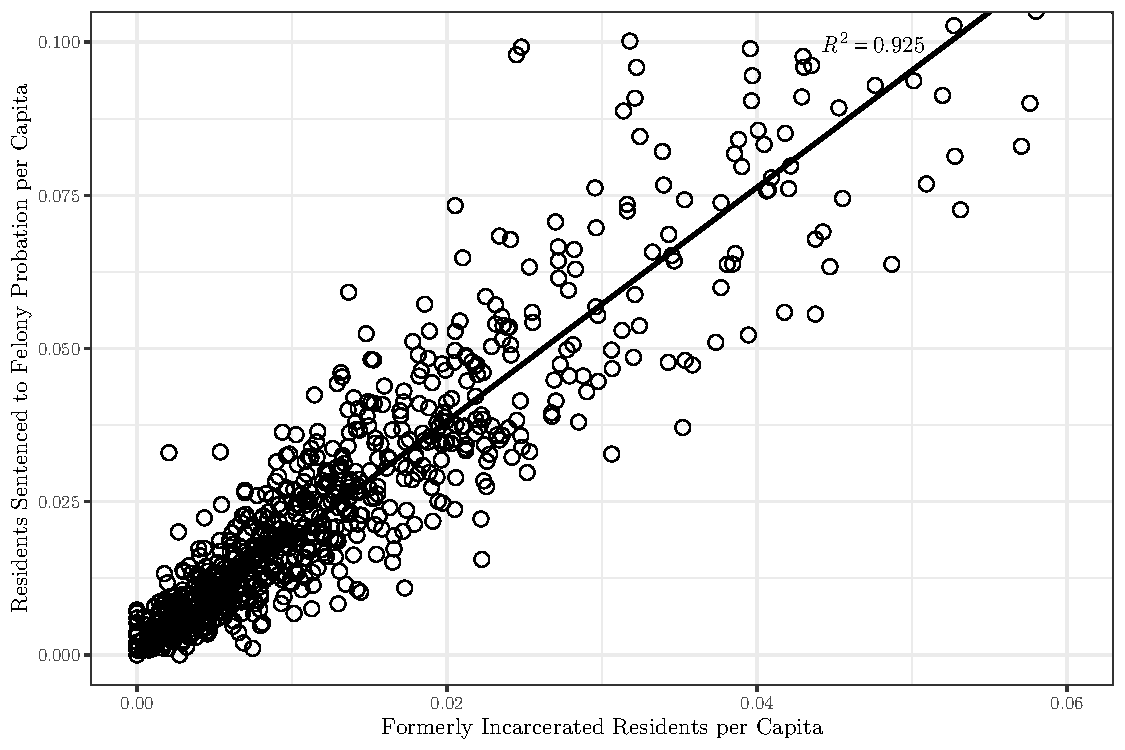
\includegraphics{SI_files/figure-latex/corrplot-1} 

}

\caption{\label{fig:scatter}Relationship Between Formerly Incarcerated and Probationed Residents, Hillsborough County}\label{fig:corrplot}
\end{figure}

Table \ref{tab:ap-hills-1} replicates the models from Tables 3 and 4 in the main body of this article. In each pair of models in the table, I begin by re-fitting the exact models presented in the body of this article but limiting the precincts and block groups to Hillsborough County. In the second model in each pair, the primary dependent variable includes both formerly incarcerated residents \emph{and} the number of residents who have been convicted of a felony probation.

\begin{singlespace}

\input{"../temp/hills_hood.tex"}
\end{singlespace}

The relationship between disenfranchised residents and precinct-level support for Amendment 4, and precinct-level turnout, are nonsignificant in Table \ref{tab:ap-hills-1} despite being significant statewide. Block group-level turnout and roll-off remain negatively associated with the presence of disenfranchised individuals. Importantly, in no model does moving from measuring only formerly incarcerated individuals to measuring all disenfranchised individuals change the sign on a statistically significant relationship. This provides corroboration for the argument that the neighborhood-level results presented in the body of this article, measured using only formerly incarcerated residents, apply to the formerly disenfranchised population more generally.

I next interrogate whether the use of only incarceration records is likely impacting the individual-level analyses presented in the body of the article. I re-run the matching procedure described above, where a registered voter is considered treated if they lived with \emph{any} disenfranchised individual. Potential controls for this matching procedure are limited to Hillsborough County, where we can be sure registered voters do not live with individuals sentenced to felony probation. The matching procedure is successful at reducing differences between treated and control voters in Hillsborough County.

In Table \ref{tab:ap-hills-2}, models 1 -- 4 re-estimate models 1 -- 4 from Table 6, where the pool is limited to treated voters who live in Hillsborough County and their matches. Models 5 -- 8 present the results using the broader treatment definition.

\begin{singlespace}
\input{"../temp/dind_reg_hills_av.tex"}
\end{singlespace}

In Hillsborough County, the magnitude of the treatment effect grows when we broaden the treatment group to include anyone who lives with a formerly disenfranchised individual. This raises interesting questions about the potential differential spillover effects of living with a formerly incarcerated individual versus with an individual sentenced to felony probation. This may also be due to some housemates of probationed individuals serving as controls in the main analysis, collapsing the distinction between treated and control and producing conservative estimates. Nonetheless, Table \ref{tab:ap-hills-2} provides evidence that the negative treatment effects identified among voters living with formerly incarcerated individuals in the body of this article are likely generalizable to all voters living with disenfranchised individuals.

\hypertarget{re-estimation-with-all-formerly-incarcerated-individuals}{%
\subsection*{Re-Estimation with All Formerly Incarcerated Individuals}\label{re-estimation-with-all-formerly-incarcerated-individuals}}
\addcontentsline{toc}{subsection}{Re-Estimation with All Formerly Incarcerated Individuals}

When discussing the impact of formerly incarcerated residents on neighborhood turnout and support for Amendment 4 in the body of this paper, I include only a subset of formerly incarcerated residents. I exclude individuals who returned from prison to institutions listed by four or more other formerly incarcerated individuals. I choose to exclude these individuals because I am most interested in the relationship between Amendment 4 and the turnout of individuals in proximal contact with the criminal justice system. Walker and García-Castañon (\protect\hyperlink{ref-Walker2017}{2017}) defines proximal contact ``as having a loved one who is a custodial citizen without yourself having had contact'' (542). Because much of the literature focuses on the mechanisms linking personal relationships, proximal contact, and political participation, I limit the sample to formerly incarcerated individuals who are likely returning to neighborhoods with social and familial ties.

Nevertheless, living in a neighborhood with a large number of formerly incarcerated individuals who reside in institutions like half-way houses or shelters might structure voting behavior. Here I re-estimate the models presented in Tables 3 and 4 in the body of this paper, but now including \emph{all} formerly incarcerated residents. Table \ref{tab:ap-a-1} presents the results of these estimations. Model 1 presents the turnout regression estimated at the block group level, while Models 2 -- 4 are estimated using precinct level data.

\begin{singlespace}

\input{"../temp/ap_a_1.tex"}
\end{singlespace}

The inclusion of all formerly incarcerated residents substantially shrinks the size of the estimated coefficients of interest with respect to the estimates presented in the body of the article. Nevertheless, turnout (measured at the block group and precinct level) and roll-off are significantly and negatively related with the formerly incarcerated population in a neighborhood, and support for Amendment 4 remains positively (and significantly) related. It appears, then, that formerly incarcerated residents who return to institutions have smaller spillover effects on their neighbors' voting behavior.

\hypertarget{re-estimation-with-recently-released-individuals}{%
\subsection*{Re-Estimation with Recently Released Individuals}\label{re-estimation-with-recently-released-individuals}}
\addcontentsline{toc}{subsection}{Re-Estimation with Recently Released Individuals}

The body of the article also acknowledges that the use of release plan address data may be unreliable considering the fact that many individuals may have moved or died since their discharge from parole. This is especially possible for individuals who have not had contact with the state incarceration agency for many years. To account for this possibility, Table \ref{tab:ap-a-2} re-estimates the models presented in Tables 3 and 4, but limits the formerly incarcerated individuals to those residents who were last released from prison between 2015 and the 2018 election. These individuals are the least likely to have died or moved, simply because their information is the most recent. These models include only individuals who returned to non-institutions, as presented in the body of the article.

\begin{singlespace}

\input{"../temp/ap_a_2.tex"}
\end{singlespace}

In each of the models presented in Table \ref{tab:ap-a-2}, the independent variable of interest is statistically significant at the 99 percent level. Moreover, the estimated coefficient is in each case larger than that presented in the body of the article. This could be because using more recent data better identifies communities that are currently home, not just historically home, to formerly incarcerated individuals. On the other hand, the primary analyses in this article indicate that a community member's incarceration may be more salient in places where residents were more recently incarcerated. Proximal contact, in other words, might shape voters' behavior more strongly if that contact was recent. The ``decaying'' spillover effects in the individual-level difference-in-differences regressions presented later in the paper would seem to corroborate this as well.

\hypertarget{refs}{}
\begin{cslreferences}
\leavevmode\hypertarget{ref-Walker2017}{}%
Walker, Hannah L., and Marcela García-Castañon. 2017. ``For Love and Justice: The Mobilizing of Race, Gender, and Criminal Justice Contact.'' \emph{Politics \& Gender} 13 (4): 541--68. \url{https://doi.org/10.1017/S1743923X17000198}.
\end{cslreferences}

\end{document}
